\documentclass{beamer}
%
% Choose how your presentation looks.
%
% For more themes, color themes and font themes, see:
% http://deic.uab.es/~iblanes/beamer_gallery/index_by_theme.html
%

\mode<presentation>
{
  \usetheme{Madrid}      % or try Darmstadt, Madrid, Warsaw, ...
  \usecolortheme{beaver} % or try albatross, beaver, crane, ...
  \usefonttheme{default}  % or try serif, structurebold, ...
  \setbeamertemplate{navigation symbols}{}
  \setbeamertemplate{caption}[numbered]
} 
\usepackage{pifont}
\usepackage[bookmarks]{hyperref}
\usepackage[backend=bibtex]{biblatex}
\usepackage{braket}
\usepackage{amsmath,amsfonts,amsthm,bm}
\addbibresource{bibliography.bib}
\newtheorem*{remark}{Remark}
\usepackage[italian]{babel}
\usepackage[utf8x]{inputenc}
\usebackgroundtemplate{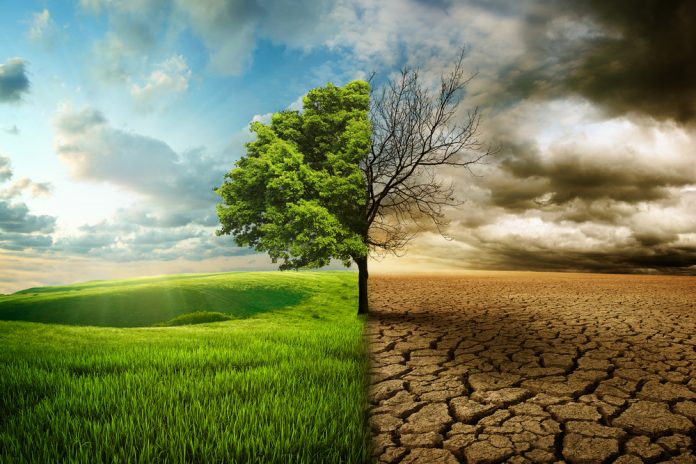
\includegraphics[width=\paperwidth]{Pic/Intro_pict.png}}
\title[Laboratorio R]{Cambiamento Climatico}
\subtitle{Laboratorio R}
\author{Marzio De Corato }
\date{\today}

\begin{document}

\begin{frame}
\vspace{+6.5 cm}  \titlepage
\end{frame}

\usebackgroundtemplate{ } 

% Uncomment these lines for an automatically generated outline.
%\begin{frame}{Outline}
%\setcounter{tocdepth}{1}
%\begin{center}
%  \tableofcontents
%\end{center}
%\end{frame}

\section{Introduzione}


\begin{frame}{Definizioni}
\begin{itemize}
\item Che cos'è il clima ? 
\end{itemize}
\end{frame}


\begin{frame}{Definizioni}
\begin{itemize}
\item Che cos'è il clima ? \textit{Sintesi statistica dei parametri atmosferici (temperatura, precipitazioni, umidità, pressione, venti) che interessano un
territorio per un periodo di tempo sufficientemente lungo} \cite{ispra}
\end{itemize}
\end{frame}


\begin{frame}{Definizioni}
\begin{itemize}
\item Che cos'è il cambiamento climatico ? 
\end{itemize}
\end{frame}

\begin{frame}{Definizioni}
\begin{itemize}
\item Che cos'è il cambiamento climatico ?  \textit{Qualsiasi cambiamento di clima attribuito direttamente o indirettamente ad attività umane, il quale altera la composizione dell'atmosfera mondiale e si aggiunge alla variabilità naturale del clima osservata in periodi di tempo comparabili} \cite{ispra}
\end{itemize}
\end{frame}




\begin{frame}{Approccio quantitativo}
\begin{itemize}
\item Come lo misuriamo ? Come lo dimostriamo ? 
\end{itemize}
\end{frame}

\begin{frame}{Approccio quantitativo}
\begin{itemize}
\item Come lo misuriamo ? Come lo dimostriamo ? 
\begin{itemize}
\item \textit{Misurazione} $\rightarrow$ \textit{serie storica (serie di osservazioni organizzate/rappresentate in ordine temporale)}
\item \textit{Significatività }
\end{itemize}
\end{itemize}
\end{frame}


\begin{frame}{Dati}
\begin{itemize}
\item Quali dati utilizziamo ?
\end{itemize}
\end{frame}

\begin{frame}{Approccio quantitativo}
\begin{itemize}
\item Quali dati utilizziamo ? 
\begin{itemize}
\item Temperatura 
\end{itemize}
\end{itemize}
\end{frame}


\begin{frame}{Approccio quantitativo}
\begin{itemize}
\item Quali dati utilizziamo ? 
\begin{itemize}
\item Temperatura  $\rightarrow$ Problema: le serie storiche affidabili di una misurazione diretta della temperatura sono disponbili dal 1880 \cite{1880}
\end{itemize}
\end{itemize}
\end{frame}

\begin{frame}{Approccio quantitativo}
\begin{itemize}
\item Quali dati utilizziamo ? 
\begin{itemize}
\item Temperatura  $\rightarrow$ Problema: le serie storiche affidabili di una misurazione diretta della temperatura sono disponbili dal 1880 \cite{1880}
\item SOLUZIONE: Uso delle misurazioni indirette: anelli di crescita degli alberi, carotaggi dei ghiacciai...
\end{itemize}
\end{itemize}
\end{frame}


\begin{frame}{Approccio quantitativo}
\begin{figure}
\begin{center}
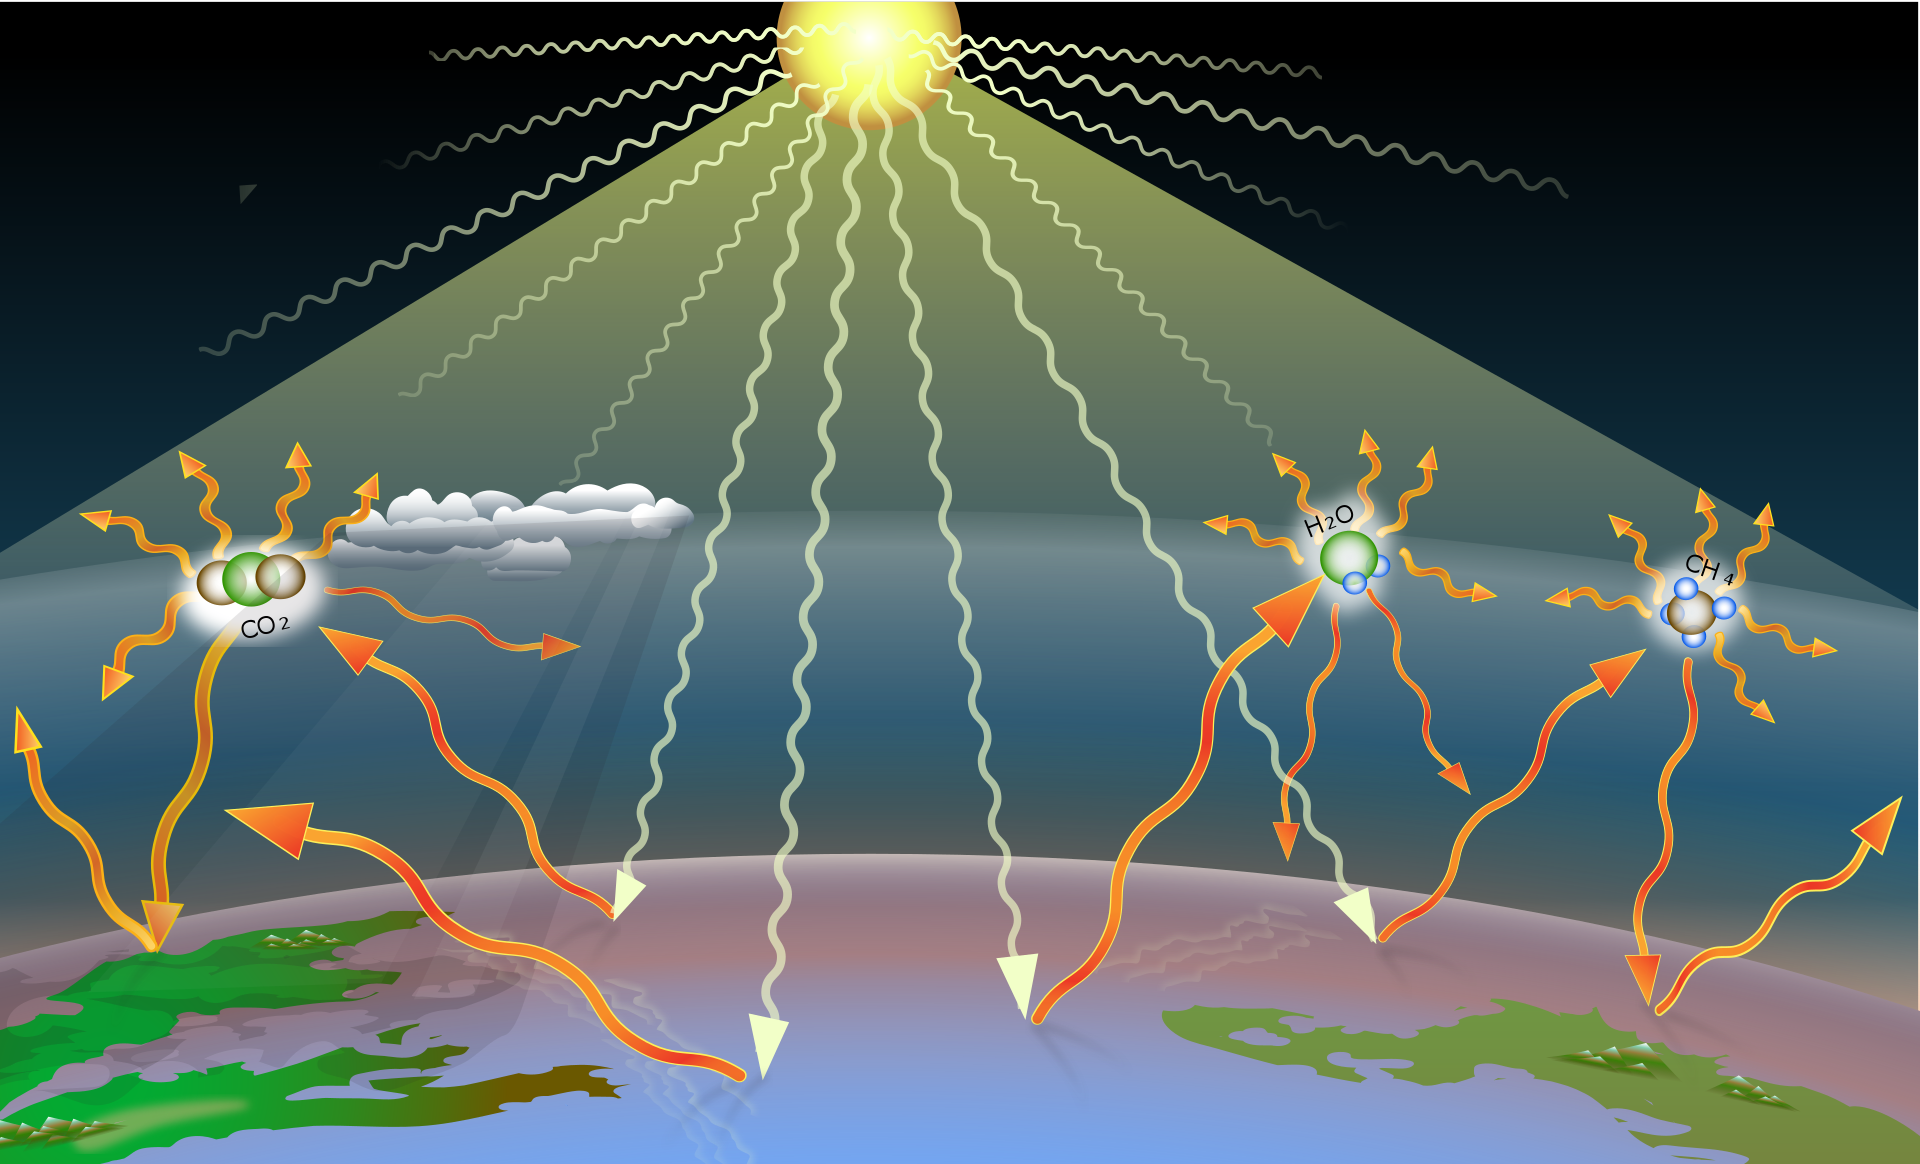
\includegraphics[width=0.7\textwidth ]{Pic/1920px-Greenhouse-effect-t2.png}
\caption{Immagine presa da \cite{wiki}}
\end{center}
\end{figure}
\end{frame}

\begin{frame}{Approccio quantitativo}
\begin{itemize}
\item Quali dati utilizziamo ? 
\begin{itemize}
\item Temperatura  $\rightarrow$ Problema: le serie storiche affidabili di una misurazione diretta della temperatura sono disponbili dal 1880 \cite{1880}
\item SOLUZIONE: Uso delle misurazioni indirette: anelli di crescita degli alberi, carotaggi dei ghiacciai...
\item Concentrazione CO$_{2}$, CH$_{4}$: le serie storiche di una misurazione diretta sono molto limitate perchè la tecnologia richiesta non è banale (e.g spettroscopia infrarossa). 
\item SOLUZIONE: carotaggi dei ghiacciai....
\item N.B vengono considerati anche altri gas
\end{itemize}
\end{itemize}
\end{frame}


\section{Ricerca dei dati}

\begin{frame}{Ricerca dei dati}
\begin{itemize}
\item Su quali fonti cercare le informazioni ? 
\item Come essere sicuri che le fonti siano attendibili ? 
\item Le fonti forniscono i raw data ? 
\end{itemize}
\end{frame}

\begin{frame}{Ricerca dei dati}
\begin{itemize}
\item Dati forniti da EPICA: European Project for Ice Coring in Antarctica (1996-2005)
\end{itemize}
\begin{figure}
\begin{center}
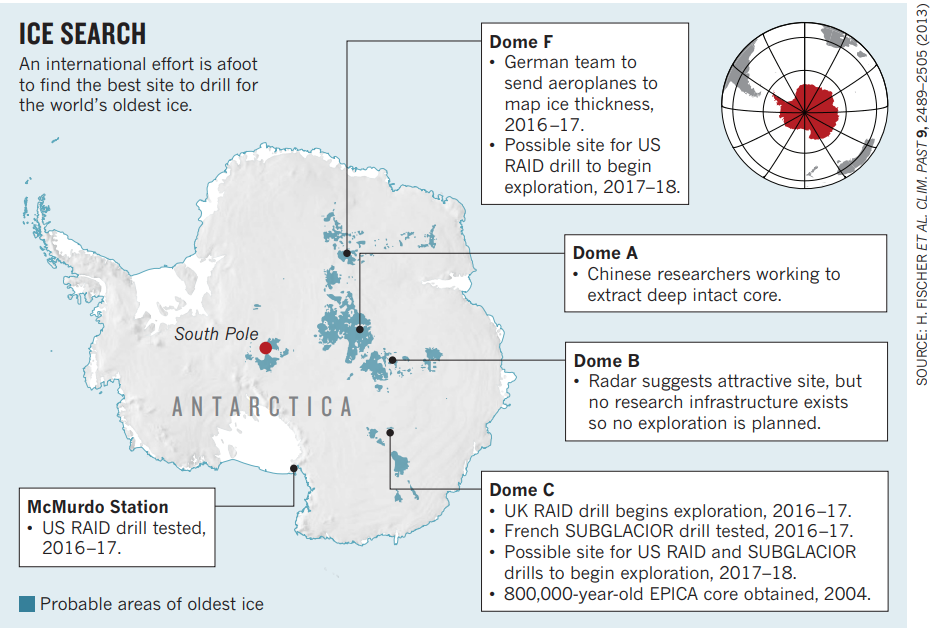
\includegraphics[width=0.7\textwidth ]{Pic/EPICAC.png}
\caption{Immagine presa da \cite{EPICAC}}
\end{center}
\end{figure}

\end{frame}


\begin{frame}{Ricerca dei dati}
\begin{figure}
\begin{center}
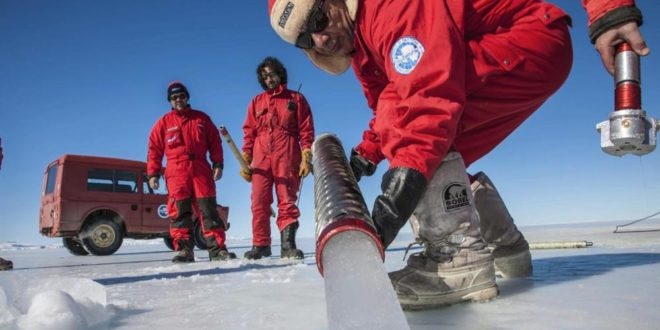
\includegraphics[width=0.7\textwidth ]{Pic/Carotaggi.jpg}
\end{center}
\end{figure}

\end{frame}


\begin{frame}{Ricerca dei dati}
\begin{center}
EPICA DOME C
\end{center}
\begin{figure}
\begin{center}
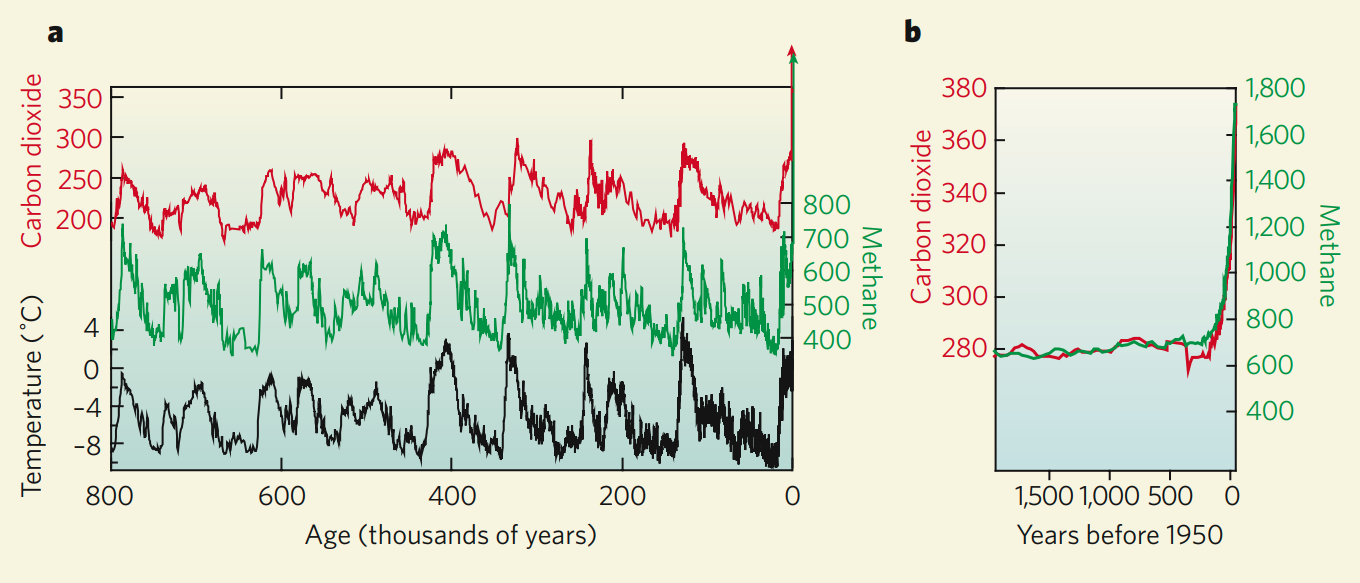
\includegraphics[width=\textwidth ]{Pic/Overview.png}
\caption{Immagine presa da \cite{overview}}
\end{center}
\end{figure}

\end{frame}


\begin{frame}{Programma esercitazione}
\begin{center}
Programma dell'esercitazione
\end{center}
\begin{itemize}
\item Ottenere i dati mostrati in precedenza
\item Analisi statistica delle serie storiche CO$_{2}$ e CH$_4$ e loro visualizzazione
\item Confronto con i valori attuali 
\end{itemize}

\end{frame}

\begin{frame}{Ricerca dei dati}
\begin{center}
Come cercare i dati ? 
\end{center}
\begin{figure}
\begin{center}
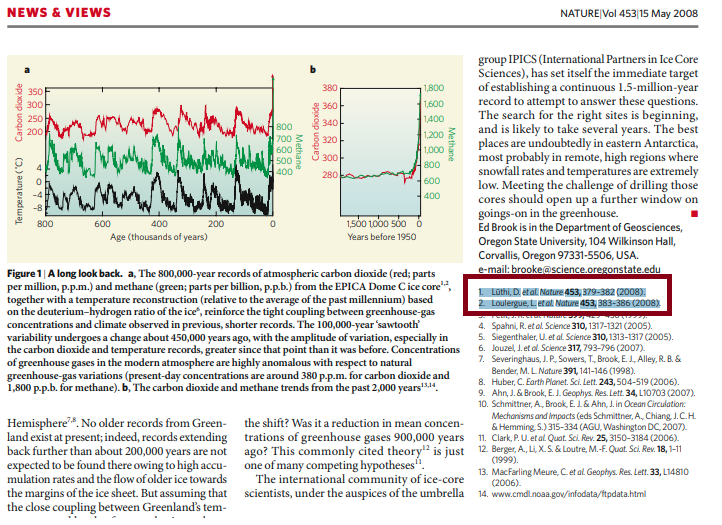
\includegraphics[width=\textwidth ]{Pic/Nature.png}
\caption{Immagine presa da \cite{overview}}
\end{center}
\end{figure}

\end{frame}




\begin{frame}{Data retrival}
\begin{itemize}
\item Scaricare i dati dal sito del \textit{National Oceanic and Atmospheric Administration} \href{https://www.ncei.noaa.gov/access/paleo-search/}{\beamergotobutton{Link}}
\end{itemize}
\end{frame}


\begin{frame}{Ricerca dei dati}
\begin{center}
Come cercare i dati ? 
\end{center}
\begin{figure}
\begin{center}
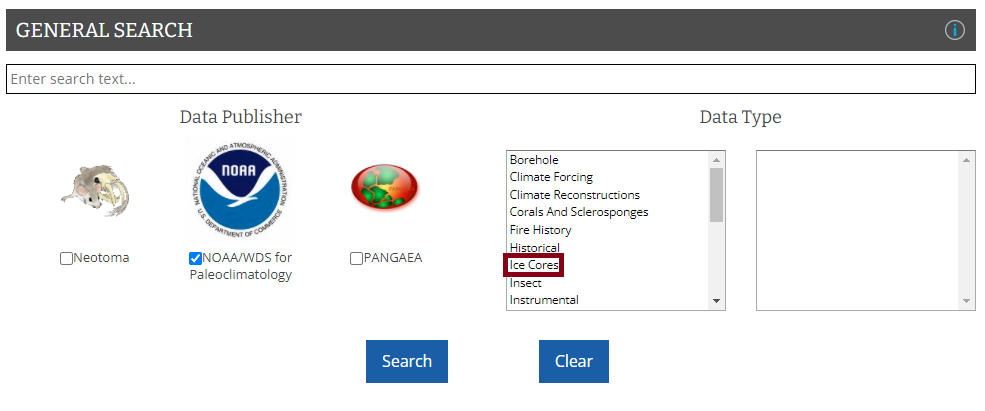
\includegraphics[width=\textwidth ]{Pic/NOAA_1.png}
\end{center}
\end{figure}
\end{frame}

\begin{frame}{Ricerca dei dati}
\begin{center}
Come cercare i dati ? 
\end{center}
\begin{figure}
\begin{center}
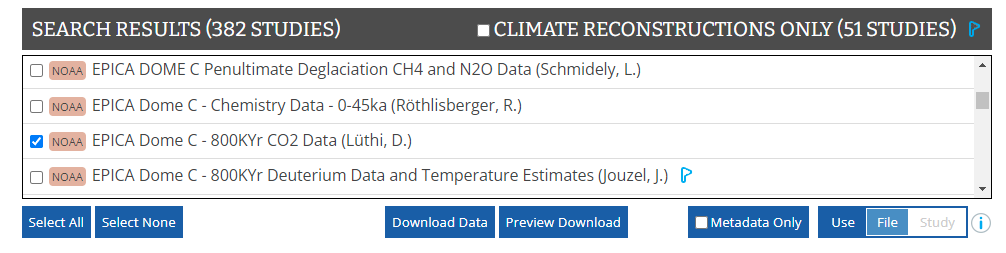
\includegraphics[width=\textwidth ]{Pic/NOAA_2.png}
\end{center}
\end{figure}
\end{frame}


\begin{frame}{Ricerca dei dati}
\begin{center}
Come cercare i dati ? 
\end{center}
\begin{figure}
\begin{center}
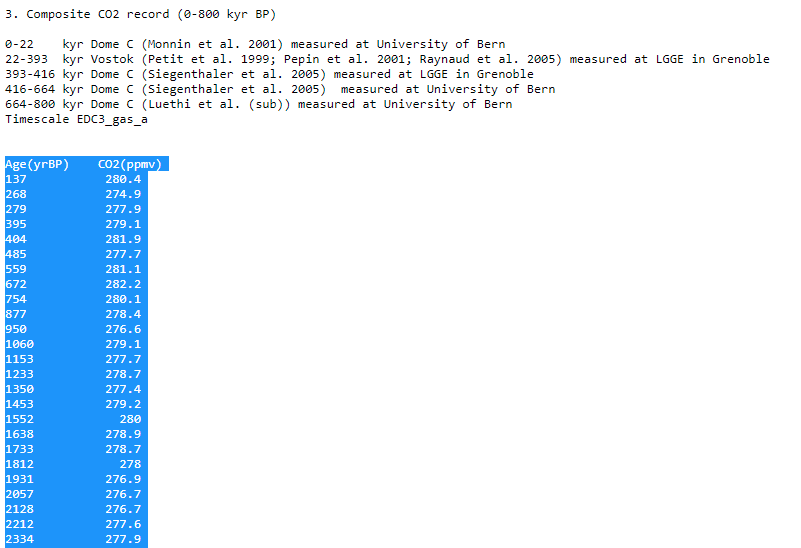
\includegraphics[width=\textwidth ]{Pic/CO2_data.png}
\end{center}
\end{figure}
\end{frame}

\begin{frame}{Ricerca dei dati}
\begin{center}
Come cercare i dati ? 
\end{center}
\begin{figure}
\begin{center}
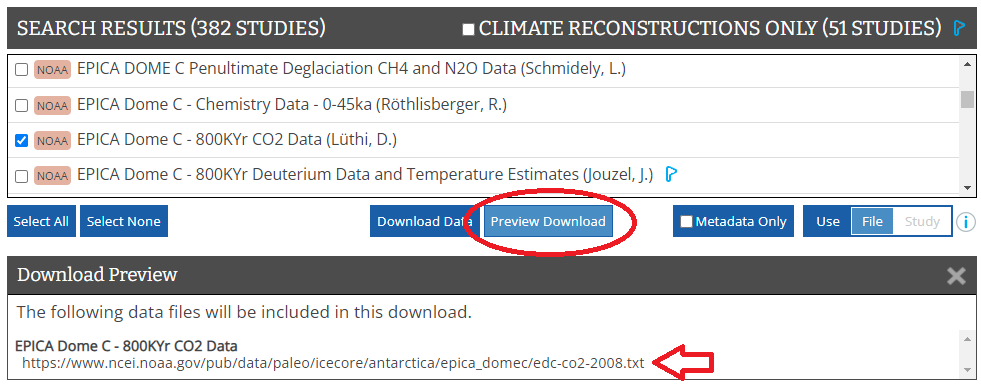
\includegraphics[width=\textwidth ]{Pic/NOAA_3.png}
\end{center}
\end{figure}
\end{frame}


\begin{frame}{Ricerca dei dati}
\begin{center}
Come cercare i dati ? 
\end{center}
\begin{figure}
\begin{center}
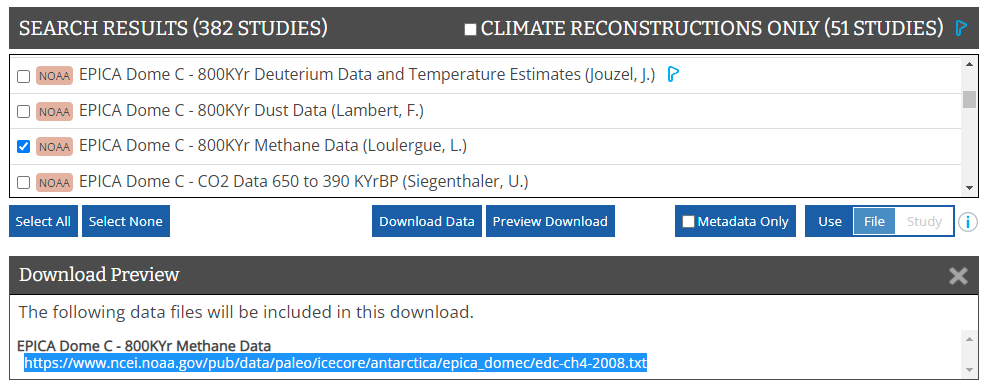
\includegraphics[width=\textwidth ]{Pic/NOAA_4.png}
\end{center}
\end{figure}
\end{frame}

\begin{frame}{Ricerca dei dati}
\begin{center}
Copiare in un txt separato il seguente campo (se ci sono spazi nelle label rimuoverli)
\end{center}
\begin{figure}
\begin{center}
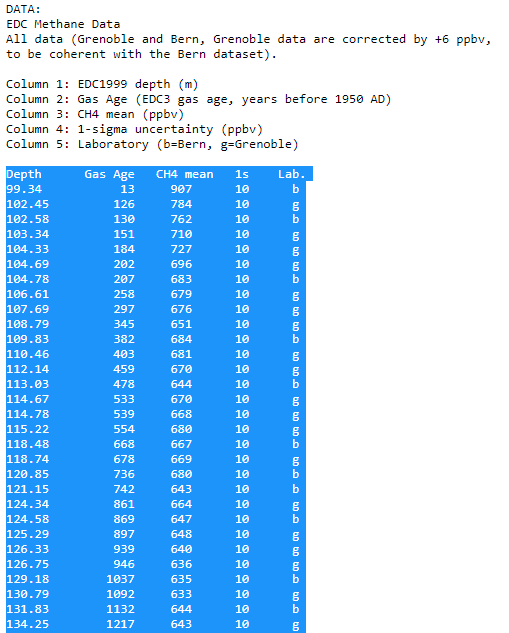
\includegraphics[width=\textwidth ]{Pic/CH4_DATA.png}
\end{center}
\end{figure}
\end{frame}


\begin{frame}{Ricerca dei dati}
\begin{itemize}
\item Scaricare i dati della concentrazione della concentrazione di CO2 dal 1959 dal sito NOAA
 \href{https://gml.noaa.gov/webdata/ccgg/trends/co2/co2_annmean_mlo.txt}{\beamergotobutton{Link}}
 
\item Fare lo stesso con la temperatura  \href{https://www.ncdc.noaa.gov/cag/global/time-series/globe/land_ocean/1/12/1959-2021}{\beamergotobutton{Link}}

\item Scaricare i dati mensili della temperatura globale da \href{https://www.metoffice.gov.uk/hadobs/hadcrut5/data/current/analysis/diagnostics/HadCRUT.5.0.1.0.analysis.summary_series.global.monthly.csv}{\beamergotobutton{Link}} (servizio meteorologico nazionale del Regno Unito)
\end{itemize}
\end{frame}

\begin{frame}{Caricamento e analisi dei dati}
\begin{center}
Fare riferimento al notebook. Assicurarsi di mettere tutti i dati scaricati (e ritagliati) in una cartella denominata Data (nella stessa directory dove è presente il notebook)
\end{center}
\end{frame}





\begin{frame}[t,allowframebreaks]
\frametitle{Bibliography}
\printbibliography
\end{frame}





\end{document}
